% Partial products of the sine formula at x=1/2, N=1..8, against the value 1.
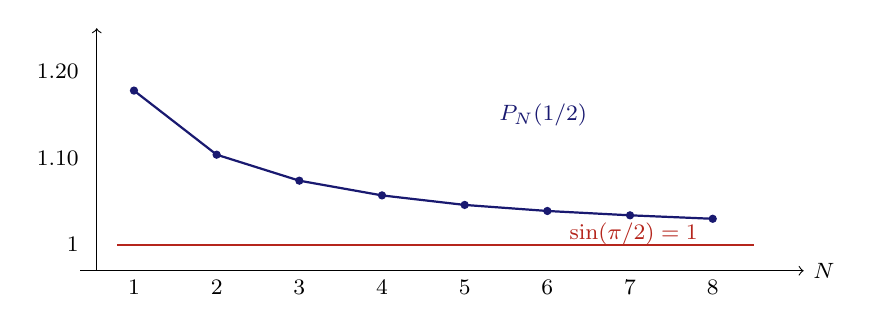
\begin{tikzpicture}[x=1.05cm,y=11cm,every node/.style={font=\footnotesize}]
  \draw[->,black] (0.35,0.02)--(9.1,0.02) node[right] {$N$};
  \draw[->,black] (0.55,0.02)--(0.55,0.30);
  \draw[BrickRed,thick] (0.8,0.05)--(8.5,0.05);
  \draw[MidnightBlue,thick] (1,0.228)--(2,0.154)--(3,0.124)--(4,0.107)--(5,0.096)--(6,0.089)--(7,0.084)--(8,0.080);
  \foreach \n/\y in {1/0.228,2/0.154,3/0.124,4/0.107,5/0.096,6/0.089,7/0.084,8/0.080} {
    \fill[MidnightBlue] (\n,\y) circle (1.5pt);
    \node[below] at (\n,0.02) {$\n$};
  }
  \node[anchor=east] at (0.45,0.05) {$1$};
  \node[anchor=east] at (0.45,0.15) {$1.10$};
  \node[anchor=east] at (0.45,0.25) {$1.20$};
  \node[BrickRed,anchor=west] at (6.15,0.062) {$\sin(\pi/2)=1$};
  \node[MidnightBlue,anchor=west] at (5.3,0.20) {$P_N(1/2)$};
\end{tikzpicture}
